\documentclass[a4paper,14pt]{extarticle}

\usepackage[utf8x]{inputenc}
\usepackage[T1,T2A]{fontenc}
\usepackage[russian]{babel}
\usepackage{hyperref}
\usepackage{indentfirst}
\usepackage{here}
\usepackage{array}
\usepackage{graphicx}
\usepackage{caption}
\usepackage{subcaption}
\usepackage{chngcntr}
\usepackage{amsmath}
\usepackage{amssymb}
\usepackage{pgfplots}
\usepackage{pgfplotstable}
\usepackage[left=2cm,right=2cm,top=2cm,bottom=2cm,bindingoffset=0cm]{geometry}
\usepackage{multicol}
\usepackage{askmaps}
\usepackage{titlesec}
\usepackage{listings}
\usepackage{color}
\usepackage{courier}

\definecolor{green}{rgb}{0,0.6,0}
\definecolor{gray}{rgb}{0.5,0.5,0.5}
\definecolor{purple}{rgb}{0.58,0,0.82}

\lstset{
	language=Verilog,
	backgroundcolor=\color{white},   
	basicstyle=\small\ttfamily,
	commentstyle=\color{green},
	keywordstyle=\color{blue},	
	numberstyle=\tiny\color{gray},
	stringstyle=\color{purple},
	breakatwhitespace=false,
	breaklines=true,
	captionpos=b,
	keepspaces=true,
	numbers=left,
	numbersep=5pt,
	showspaces=false,
	showstringspaces=false,
	showtabs=false,
	tabsize=4,
	frame=single,
	inputpath={../quartus/},
	literate={~} {$\sim$}{1}
}

\renewcommand{\le}{\ensuremath{\leqslant}}
\renewcommand{\leq}{\ensuremath{\leqslant}}
\renewcommand{\ge}{\ensuremath{\geqslant}}
\renewcommand{\geq}{\ensuremath{\geqslant}}
\renewcommand{\epsilon}{\ensuremath{\varepsilon}}
\renewcommand{\phi}{\ensuremath{\varphi}}
\renewcommand{\thefigure}{\arabic{figure}} 	
\renewcommand*\not[1]{\overline{#1}}

\titleformat*{\section}{\large\bfseries} 
\titleformat*{\subsection}{\normalsize\bfseries} 
\titleformat*{\subsubsection}{\normalsize\bfseries} 
\titleformat*{\paragraph}{\normalsize\bfseries} 
\titleformat*{\subparagraph}{\normalsize\bfseries} 

\counterwithin{figure}{section}
\counterwithin{equation}{section}
\counterwithin{table}{section}
\newcommand{\sign}[1][5cm]{\makebox[#1]{\hrulefill}}
\graphicspath{{../pics/}}
\captionsetup{justification=centering,margin=1cm}
\def\arraystretch{1.3}
\setlength\parindent{5ex}
\titlelabel{\thetitle.\quad}

\begin{document}

\begin{titlepage}
\begin{center}
	Санкт-Петербургский Политехнический Университет Петра Великого\\[0.3cm]
	Институт компьютерных наук и технологий \\[0.3cm]
	Кафедра компьютерных систем и программных технологий\\[4cm]
	
	\textbf{ОТЧЕТ}\\ 
	\textbf{по лабораторной работе}\\[0.5cm]
	\textbf{SystemVerilog №4}\\[0.1cm]
	Автоматизация проектирования\\ дискретных устройств\\[4.0cm]
\end{center}

\begin{flushright}
	\begin{minipage}{0.45\textwidth}
		\textbf{Работу выполнил студент}\\[3mm]
		группа 33501/4 \hspace*{9mm} Дьячков В.В.\\[5mm]
		\textbf{Преподаватель}\\[5mm]
		\sign[1.5cm] \hspace*{1mm} к.т.н., доц. Филиппов А.С. \\[5mm]
	\end{minipage}
\end{flushright}

\vfill

\begin{center}
	Санкт-Петербург\\
	\the\year
\end{center}
\end{titlepage}

\addtocounter{page}{1}
\counterwithin{lstlisting}{section}

\tableofcontents
\newpage
\listoffigures
\lstlistoflistings
\newpage

\section{lab5\_1}

\subsection{Задание}

На языке Verilog опишите параметризированное устройство для выполнения bitwise операций. 
\begin{itemize}
	\item Параметры:
		\begin{itemize}
			\item \code{N} – разрядность операндов и результата (базовое значение 4).
			\item \code{LOGIC_TYPE} -- код логической операции 
				\begin{enumerate}
					\setcounter{enumi}{-1}
					\item \code{&}
					\item \code{|}
					\item \code{^}
				\end{enumerate}
			\item \code{IN_A_NOT} -- инверсия операнда А ($=1$ -- инверсия).
			\item \code{IN_B_NOT} -- инверсия операнда B ($=1$ -- инверсия).
			\item \code{OUT_NOT} -- инверсия выхода ($=1$ -- инверсия).		
		\end{itemize}
	\item Входы:
		\begin{itemize}
			\item Переключатели \code{sw[3:0]} -- операнд А;
			\item Переключатели \code{sw[7:4]} -- операнд В.
		\end{itemize}
	\item Выходы: светодиоды \code{led[7:4]}.
\end{itemize}

Дополнительные требования:
\begin{itemize}
	\item[$\circ$] Стандарты и номера выводов СБИС для платы miniDiLaB\_CIV задать с помощью атрибутов.
	\item[$\circ$] Счетчик-делитель и автомат описываются в отдельных процедурных блоках.
	\item[$\circ$] Осуществите функциональное моделирование (и приведите в отчете результаты) при:
		\begin{itemize}
			\item \code{N = 4};
			\item \code{LOGIC_TYPE} -- все возможные значения;
			\item \code{IN_A_NOT = 0};
			\item \code{IN_B_NOT = 1};
			\item \code{OUT_NOT = 0}.
		\end{itemize}
	\item[$\circ$] Проверку на плате осуществите при:
		\begin{itemize}
			\item \code{N = 4};
			\item \code{LOGIC_TYPE} -- все возможные значения;
			\item \code{IN_A_NOT = 0}; 
			\item \code{IN_B_NOT = 1};
			\item \code{OUT_NOT = 1}.
		\end{itemize}
\end{itemize}
В описании можно использовать любые операторы.

\subsection{Код на языке Verilog}

В листинге \ref{code:1} приведен код программы на языке Verilog.

\lstinputlisting[caption=lab5\_1.v, label=code:1]{lab5_1/lab5_1.v}

\subsection{Результаты синтеза}

На рис. \ref{fig:lab5_1_rtl} приведено изображение синтезированной схемы в RLT Viewer.

\begin{figure}[H]
\begin{center}
	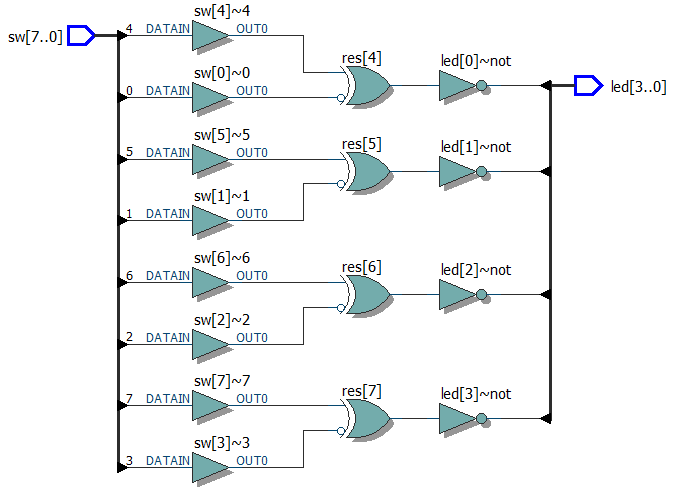
\includegraphics[width=0.7\textwidth]{lab5_1_rtl}
	\caption{Результат синтеза в RLT Viewer}
	\label{fig:lab5_1_rtl}
\end{center}
\end{figure}

\subsection{Результаты моделирования}
\label{sec:lab5_1_modeling}

На рис. \ref{fig:lab5_1_modeling_1} -- \ref{fig:lab5_1_modeling_3} изображены временная диаграмма работы синтезированного устройства при \code{LOGIC_TYPE} равным \code{&}, \code{|} и \code{^} соответственно.
\vspace{-0.2cm}
\begin{figure}[H]
\begin{center}
	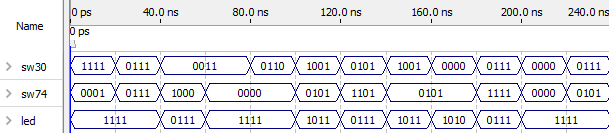
\includegraphics[width=\textwidth]{lab5_1_modeling_1}
	\caption{Результаты моделирования при \code{LOGIC_TYPE = "&"}}
	\label{fig:lab5_1_modeling_1}
\end{center}
\end{figure}
\vspace{-0.5cm}
\begin{figure}[H]
\begin{center}
	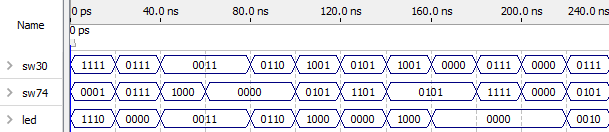
\includegraphics[width=\textwidth]{lab5_1_modeling_2}
	\caption{Результаты моделирования при \code{LOGIC_TYPE = "|"}}
	\label{fig:lab5_1_modeling_2}
\end{center}
\end{figure}
\begin{figure}[H]
\begin{center}
	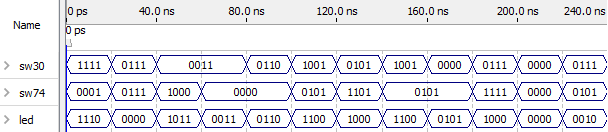
\includegraphics[width=\textwidth]{lab5_1_modeling_3}
	\caption{Результаты моделирования при \code{LOGIC_TYPE = "^"}}
	\label{fig:lab5_1_modeling_3}
\end{center}
\end{figure}

\subsection{Назначение выводов СБИС}

На рис. \ref{fig:lab5_1_pins} приведены назначения выводов СБИС в Pin Planner.

\begin{figure}[H]
\begin{center}
	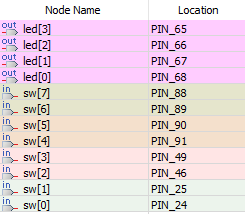
\includegraphics{lab5_1_pins}
	\caption{Таблица назначений в Pin Planer}
	\label{fig:lab5_1_pins}
\end{center}
\end{figure}

\subsection{Результаты проверки на плате}

Для тестирования проекта на плате были использованы значения  \code{N = 4}, \code{LOGIC_TYPE} -- все возможные значения, \code{IN_A_NOT = 0}, \code{IN_B_NOT = 1} и \code{OUT_NOT = 1}. Результаты тестирования совпадают с ожидаемыми, следовательно, устройство работает верно.

\subsection{Выводы}

Реализовано параметризированное устройство для выполнения bitwise операций. Результаты моделирования и тестирования на плате показали, что разработанное устройство работает верно.

\section{lab5\_2}

\subsection{Задание}

На языке Verilog опишите устройство, включающее:
\begin{itemize}
	\item Счетчик-делитель, обеспечивает счет по модулю \code{N} (базовое значение -- \code{3}) и формирование синхронного сигнала переноса (активный уровень сигнала -- \code{1}, длительность один такт тактовой частоты) по достижению счетчиком значения \code{N-1}.
	\item Конечный автомат, граф переходов которого приведен на рис \ref{fig:lab5_2_0}.
		\vspace{-0.5cm}
		\begin{figure}[H]
		\begin{center}
			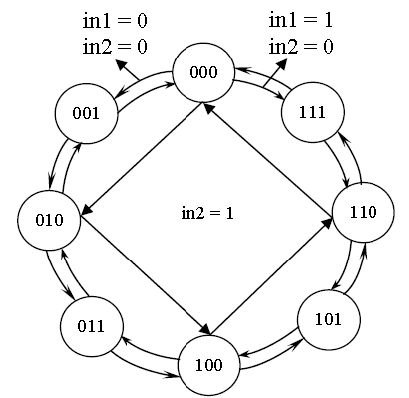
\includegraphics[scale=0.7]{lab5_2_0}
			\caption{Конечный автомат}
			\label{fig:lab5_2_0}
		\end{center}
		\end{figure}
		\vspace{-1cm}
		\begin{itemize}
			\item В узлах автомата указано значение выходов автомата;
			\item \code{in1}, \code{in2} – входные сигналы автомата;
			\item Имена состояний автомата выбираются самостоятельно;
			\item Автомат имеет вход асинхронного сброса (сигнал \code{rst}) в состояние, в котором выходные сигналы \code{000}: при \code{rst = 0} – асинхронный сброс;
			\item Автомат имеет вход разрешения работы -- \code{ena} (при \code{ena = 1} – работа разрешена), подключенный к сигналу переноса счетчика-делителя.
		\end{itemize}	
	\item Входы:
		\begin{itemize}
			\item Переключатель \code{sw[1]} -- вход \code{in1};
			\item Переключатель \code{sw[2]} – вход \code{in2};
			\item Кнопка \code{pba} – вход асинхронного сброса (кнопка нажата -- сброс);
			\item Тактовый сигнал (\code{clk}) подается от тактового генератора (см. описание стенда). Частота тактового сигнала – 25МГц.
		\end{itemize}		
	\item Выходы: светодиоды \code{led[2:0]} -- выходы автомата.
\end{itemize}

Дополнительные требования:
\begin{itemize}
	\item[$\circ$] Стандарты и номера выводов СБИС для платы miniDiLaB\_CIV задать с помощью атрибутов.
	\item[$\circ$] При моделировании устройства, с целью сокращения времени моделирования, для счетчика-делителя установите параметр \code{N} равным \code{3} (а не \code{25 000 000}).
	\item[$\circ$] При функциональном моделировании автомата проверьте все состояния и переход по всем ребрам графа.
\end{itemize}

В описании можно использовать любые операторы.

\subsection{Код на языке Verilog}

В листинге \ref{code:2} приведен код программы на языке Verilog.

\lstinputlisting[caption=lab5\_2.v, label=code:2]{lab5_2/lab5_2.v}
\vspace{-0.5cm}

\subsection{Результаты синтеза}

На рис. \ref{fig:lab5_2_rtl} приведено изображение синтезированной схемы в RLT Viewer.

\begin{figure}[H]
\begin{center}
	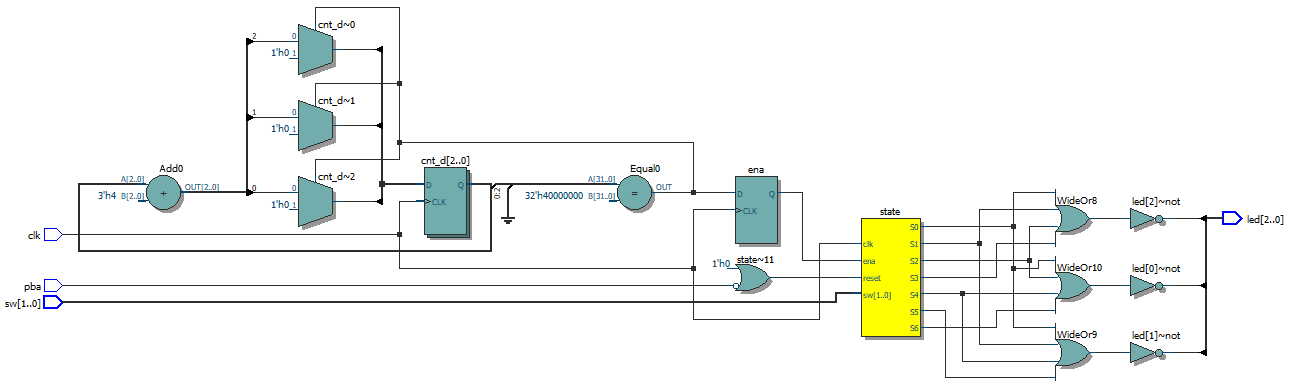
\includegraphics[width=\textwidth]{lab5_2_rtl}
	\caption{Результат синтеза в RLT Viewer}
	\label{fig:lab5_2_rtl}
\end{center}
\end{figure}

\newpage

\subsection{Результаты моделирования}
\label{sec:lab5_2_modeling}

На рис. \ref{fig:lab5_2_modeling} изображена временная диаграмма работы синтезированного устройства.

\begin{figure}[H]
\begin{center}
	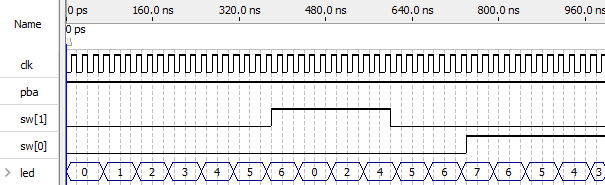
\includegraphics[width=\textwidth]{lab5_2_modeling}
	\caption{Результаты моделирования}
	\label{fig:lab5_2_modeling}
\end{center}
\end{figure}

\subsection{Назначение выводов СБИС}

На рис. \ref{fig:lab5_2_pins} приведены назначения выводов СБИС в Pin Planner.

\begin{figure}[H]
\begin{center}
	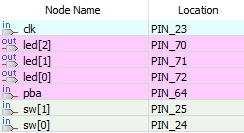
\includegraphics{lab5_2_pins}
	\caption{Таблица назначений в Pin Planer}
	\label{fig:lab5_2_pins}
\end{center}
\end{figure}

\subsection{Результаты проверки на плате}

Для тестирования проекта на плате были использованы тесты, описанные в пункте \ref{sec:lab5_2_modeling}. Результаты тестирования совпадают с ожидаемыми, следовательно, устройство работает верно.

\subsection{Выводы}

Реализовано устройство, содержащее счетчик-делитель и конечный автомат. Результаты моделирования и тестирования на плате показали, что разработанное устройство работает верно.

\newpage

\section{elab5\_1}

\subsection{Задание}

На языке Verilog опишите устройство, включающее:
\begin{itemize}
	\item Два входа операндов (\code{op_a}, \code{op_b}) -- операнды без знаковые.
	\item Вход кода операции (\code{op}).
	\item Выход результата (\code{res}).
	\item Выход переполнения (\code{over}).
	\item Параметр: \code{N} -- разрядность операндов и результата (базовое значение 3).
	\item Локальный параметр: \code{code_op} -- код операции.
	\vspace{-0.5cm}
	\begin{table}[H]
	\begin{center}
		\def\tabcolsep{10pt}
		\caption{Коды операций}
		\begin{tabular}{|c|c|c|c|c|}
		\hline	
		\makecell{Обозначение \\ кода операции} & \makecell{Значение \\ кода операции} & Операция \\ 
		\hline
		\code{ZERO} & \code{00} & \code{res = 0} \\
		\hline
		\code{SUM} & \code{01} & \code{res = op_a + op_b} \\
		\hline
		\code{SUB} & \code{10} & \code{res = op_a - op_b} \\
		\hline
		\code{MULT} & \code{11} & На выходе большее из \code{op_a} и \code{op_b} \\
		\hline
		\end{tabular}
	\end{center}
	\end{table}	
	\vspace{-0.5cm}
	\item Входы:
		\begin{itemize}
			\item Переключатели \code{sw[2:0]} -- операнд А (\code{op_a})
			\item Переключатели \code{sw[5:3]} -- операнд В (\code{op_b})
			\item Переключатели \code{sw[7:6]} -- код операции (\code{op})
		\end{itemize}
	\item Выходы:
		\begin{itemize}
			\item Светодиоды \code{led[2:0]} -- выход результата (\code{res});
			\item светодиод \code{led[3]} -- выход переполнения (\code{over}).
		\end{itemize}
\end{itemize}

Дополнительные требования:
\begin{itemize}
	\item[$\circ$] Стандарты и номера выводов СБИС для платы miniDiLaB\_CIV задать с помощью атрибутов.
	\item[$\circ$] Осуществите функциональное моделирование (и приведите в отчете результаты) при \code{N = 8}.
	\item[$\circ$] Проверку на плате осуществите при \code{N = 3}.
\end{itemize}

В описании можно использовать любые операторы.

\subsection{Код на языке Verilog}

В листинге \ref{code:5} приведен код программы на языке Verilog.

\lstinputlisting[caption=elab5\_1.v, label=code:5]{elab5_1/elab5_1.v}

\newpage

\subsection{Результаты синтеза}

На рис. \ref{fig:elab5_1_rtl} приведено изображение синтезированной схемы в RLT Viewer.

\begin{figure}[H]
\begin{center}
	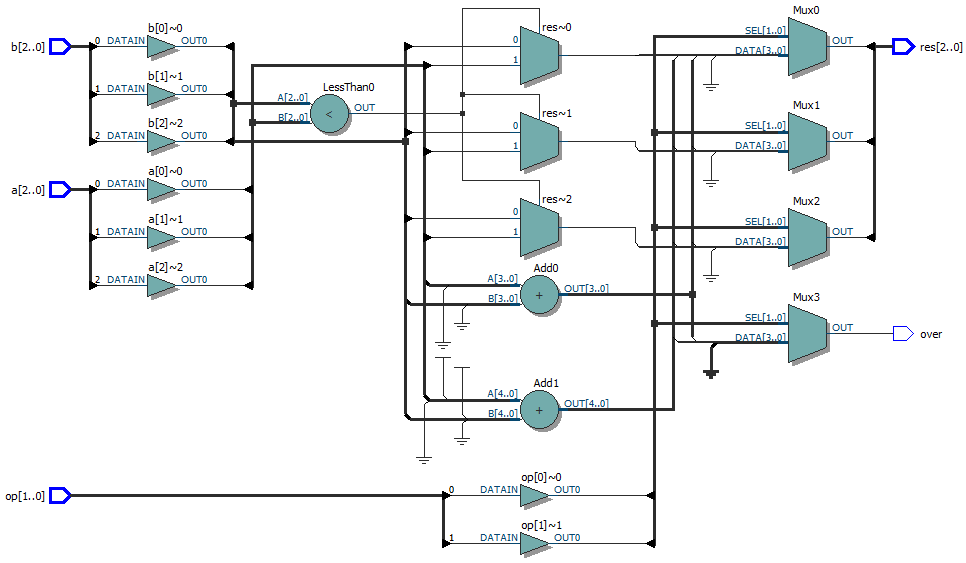
\includegraphics[width=\textwidth]{elab5_1_rtl}
	\caption{Результат синтеза в RLT Viewer}
	\label{fig:elab5_1_rtl}
\end{center}
\end{figure}

\subsection{Результаты моделирования}
\label{sec:elab5_1_modeling}

На рис. \ref{fig:elab5_1_modeling} изображена временная диаграмма работы синтезированного устройства. 

\begin{figure}[H]
\begin{center}
	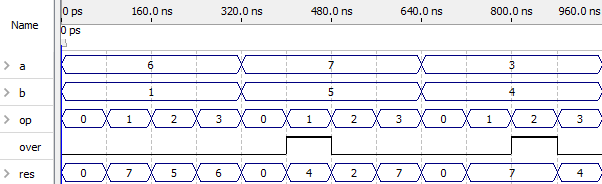
\includegraphics[width=\textwidth]{elab5_1_modeling}
	\caption{Результаты моделирования}
	\label{fig:elab5_1_modeling}
\end{center}
\end{figure}

\subsection{Назначение выводов СБИС}

На рис. \ref{fig:elab5_1_pins} приведены назначения выводов СБИС в Pin Planner.

\begin{figure}[H]
\begin{center}
	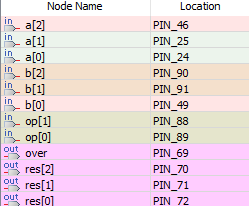
\includegraphics{elab5_1_pins}
	\caption{Таблица назначений в Pin Planer}
	\label{fig:elab5_1_pins}
\end{center}
\end{figure}

\subsection{Результаты проверки на плате}

Для тестирования проекта на плате были использованы тесты, описанные в пункте \ref{sec:elab5_1_modeling}. Результаты тестирования совпадают с ожидаемыми, следовательно, устройство работает верно.

\subsection{Выводы}

Реализовано устройство, принимающее на вход два операнда и код операции и вычисляющее результат. Результаты моделирования и тестирования на плате показали, что разработанное устройство работает верно.

\newpage

\section{elab5\_2}

\subsection{Задание}

На языке Verilog опишите устройство, включающее:
\begin{itemize}
	\item Счетчик-делитель, обеспечивает счет по модулю \code{N} (базовое значение -- 3) и формирование синхронного сигнала переноса (активный уровень сигнала -- 1, длительность один такт тактовой частоты) по достижению счетчиком значения \code{N-1}.
	\item Модуль, алгоритм которого задан графом переходов на рис. \ref{fig:lab5_2_0}.
		\begin{itemize}
			\item \code{in1}, \code{in2} -- входные сигналы модуля;
			\item Модуль имеет вход асинхронного сброса (сигнал \code{rst}) в состояние, в котором выходные сигналы \code{000}: при \code{rst=0} -- асинхронный сброс;
			\item Модуль имеет вход разрешения работы -- \code{ena} (при \code{ena=1} -- работа разрешена), подключенный к сигналу переноса счетчика-делителя.
		\end{itemize}
	\item Входы:
		\begin{itemize}
			\item Переключатель \code{sw[1]} -- вход \code{in1};
			\item Переключатель \code{sw[2]} – вход \code{in2};
			\item Кнопка \code{pba} – вход асинхронного сброса (кнопка нажата – сброс);
			\item Тактовый сигнал (\code{clk}) подается от тактового генератора (см. описание стенда). Частота тактового сигнала – 25МГц.
		\end{itemize}
	\item Выходы: светодиоды \code{led[2:0]} -- выходы модуля.
\end{itemize}

Дополнительные требования:
\begin{itemize}
	\item[$\circ$] Стандарты и номера выводов СБИС для платы miniDiLaB\_CIV задать с помощью атрибутов.
	\item[$\circ$] При моделировании устройства, с целью сокращения времени моделирования, для счетчика-делителя установите параметр \code{N} равным \code{3} (а не \code{25 000 000}).
\end{itemize}

В описании можно использовать любые операторы.

\newpage

\subsection{Код на языке Verilog}

В листинге \ref{code:5} приведен код программы на языке Verilog.

\lstinputlisting[caption=elab5\_1.v, label=code:5]{elab5_2/elab5_2.v}

\subsection{Результаты синтеза}

На рис. \ref{fig:elab5_2_rtl} приведено изображение синтезированной схемы в RLT Viewer.

\begin{figure}[H]
\begin{center}
	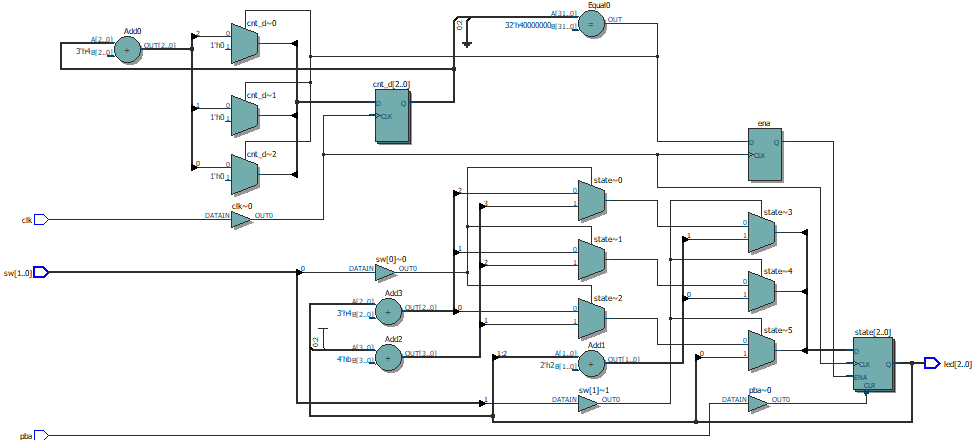
\includegraphics[width=\textwidth]{elab5_2_rtl}
	\caption{Результат синтеза в RLT Viewer}
	\label{fig:elab5_2_rtl}
\end{center}
\end{figure}

\subsection{Результаты моделирования}
\label{sec:elab5_2_modeling}

На рис. \ref{fig:elab5_2_modeling} изображена временная диаграмма работы синтезированного устройства. 

\begin{figure}[H]
\begin{center}
	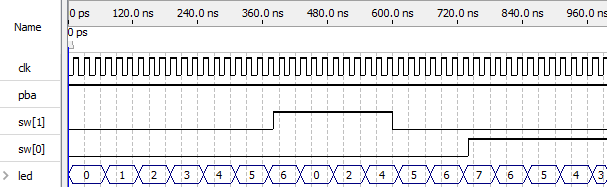
\includegraphics[width=\textwidth]{elab5_2_modeling}
	\caption{Результаты моделирования}
	\label{fig:elab5_2_modeling}
\end{center}
\end{figure}

\newpage

\subsection{Назначение выводов СБИС}

На рис. \ref{fig:elab5_2_pins} приведены назначения выводов СБИС в Pin Planner.

\begin{figure}[H]
\begin{center}
	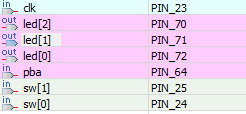
\includegraphics{elab5_2_pins}
	\caption{Таблица назначений в Pin Planer}
	\label{fig:elab5_2_pins}
\end{center}
\end{figure}

\subsection{Результаты проверки на плате}

Для тестирования проекта на плате были использованы тесты, описанные в пункте \ref{sec:elab5_2_modeling}. Результаты тестирования совпадают с ожидаемыми, следовательно, устройство работает верно.

\subsection{Выводы}

Реализовано устройство, принимающее на вход два операнда и код операции и вычисляющее результат. Результаты моделирования и тестирования на плате показали, что разработанное устройство работает верно.

\end{document}